\section{esercizio 25}

\textit{\textbf{Descrizione:}  Sia data la matrice di Toeplitz simmetrica $A_{N}$ in cui le extra-diagonali pi\'u esterne sono le none. Partendo dal vettore $\underline{u}_{0} = (1, \cdots,1)^{T} \in \mathbb{R}^{N}$, applicare il metodo delle potenze con tolleranza $tol=10^{-10}$ per $N=10:10:500$, utilizzando la function dell'esercizio 24. Graficare il valore dell'autovalore dominante, e del numero di iterazioni necessarie per soddisfare il criterio di arresto, rispetto ad N. Utilizzare la funzione spdiags di Matlab per creare la matrice e memorizzarla come matrice sparsa.}

\noindent\emph{Soluzione: }\newline
\section*{metodo delle potenze}
\lstinputlisting{resources/potenzecount.m}\newpage
\lstinputlisting{resources/es25.m}
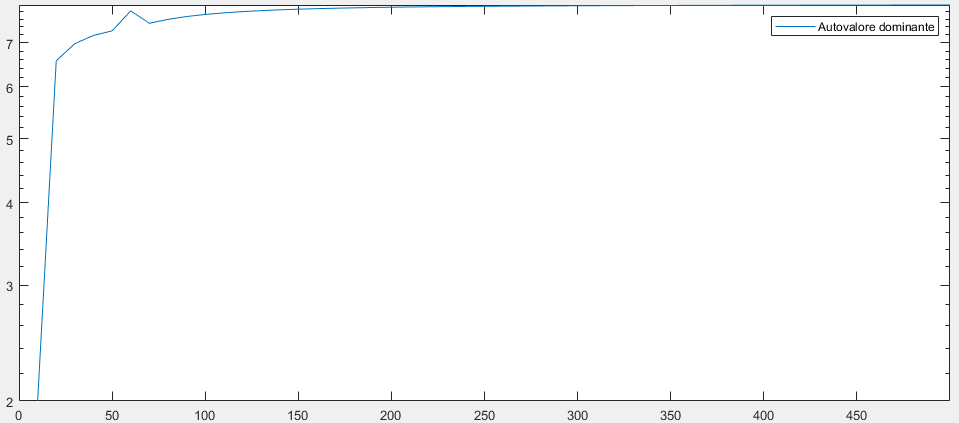
\includegraphics[width=1\linewidth]{img/autovalore.png}
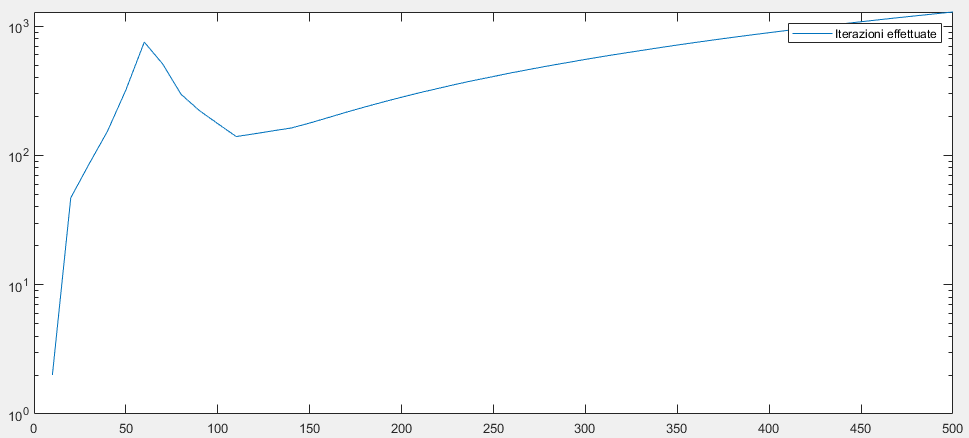
\includegraphics[width=1\linewidth]{img/iterazioniPotenze.png}
